% wpipe - Python Pipeline Library Documentation
% Professional LaTeX Document for Word Compatibility
\documentclass[12pt,a4paper]{report}

% Fuentes CRÍTICAS para compatibilidad Word
\usepackage[utf8]{inputenc}
\usepackage[T1]{fontenc}
\usepackage{helvet}
\usepackage{courier}
\usepackage{pdfpages}
\usepackage{etoolbox}
\usepackage{iftex}
\usepackage{ifplatform}

% Paquetes esenciales
\usepackage{tocbibind}
\usepackage{microtype}
\usepackage{geometry}
\usepackage{graphicx}
\usepackage{fancyhdr}
\usepackage{hyperref}
\usepackage{listings}
\usepackage{xcolor}
\usepackage{appendix}
\usepackage{float}
\usepackage{caption}
\usepackage{subcaption}
\usepackage{amsmath}
\usepackage{amssymb}
\usepackage{booktabs}
\usepackage{multirow}
\usepackage{enumitem}
\usepackage{titlesec}
\usepackage{pdflscape}
\usepackage{longtable}
\usepackage[nottoc,notlot,notlof]{tocbibind}

% Configuración de márgenes
\geometry{
    left=2.5cm,
    right=2.5cm,
    top=2.5cm,
    bottom=2.5cm,
    headheight=15pt
}

% Configuración listings EXACTA para código
\lstset{
    basicstyle=\ttfamily\footnotesize\fontfamily{pcr}\selectfont,
    backgroundcolor=\color{gray!10},
    frame=single,
    frameround=tttt,
    rulecolor=\color{gray!50},
    numbers=left,
    numberstyle=\tiny\color{gray},
    keywordstyle=\color{blue}\bfseries,
    commentstyle=\color{green!60!black}\itshape,
    stringstyle=\color{red},
    showstringspaces=false,
    breaklines=true,
    breakatwhitespace=true,
    tabsize=2,
    captionpos=b,
    xleftmargin=2em,
    framexleftmargin=1.5em,
    belowskip=1em,
    aboveskip=1em,
    language=Python
}

% Headers y footers con sans-serif
\pagestyle{fancy}
\fancyhf{}
\fancyhead[L]{\color{blue!70!black}\textbf{\sffamily\leftmark}}
\fancyhead[R]{\color{blue!70!black}\textbf{\sffamily\thepage}}
\fancyfoot[C]{\color{gray}\small\sffamily wpipe - Python Pipeline Library}
%\renewcommand{\headrulewidth}{0.4pt}
%\renewcommand{\footrulewidth}{0.4pt}

% Estilos de capítulos y secciones con sans-serif
\titleformat{\chapter}[display]
{\normalfont\huge\bfseries\sffamily\color{blue!70!black}}
{\chaptertitlename\ \thechapter}{20pt}{\Huge}
\titlespacing*{\chapter}{0pt}{-30pt}{20pt}

\titleformat{\section}
{\normalfont\Large\bfseries\sffamily\color{blue!70!black}}
{\thesection}{1em}{}
\titlespacing*{\section}{0pt}{15pt}{10pt}

\titleformat{\subsection}
{\normalfont\large\bfseries\sffamily\color{orange!80!black}}
{\thesubsection}{1em}{}
\titlespacing*{\subsection}{0pt}{10pt}{5pt}

\titleformat{\subsubsection}
{\normalfont\normalsize\bfseries\sffamily\color{gray!50!black}}
{\thesubsubsection}{1em}{}
\titlespacing*{\subsubsection}{0pt}{8pt}{4pt}

% Configuración hyperref
\hypersetup{
    colorlinks=true,
    linkcolor=blue!70!black,
    filecolor=blue!70!black,
    urlcolor=blue!70!black,
    citecolor=orange!80!black,
    pdftitle={wpipe - Python Pipeline Library for Sequential Data Processing},
    pdfauthor={William Steve Rodriguez Villamizar},
    pdfsubject={Python, Pipeline, Data Processing, MLOps},
    pdfkeywords={Python, Pipeline, Data Processing, ETL, Workflow}
}

% Colores personalizados
\definecolor{primary}{RGB}{102, 126, 234}
\definecolor{secondary}{RGB}{118, 75, 162}
\definecolor{accent}{RGB}{255, 107, 107}
\definecolor{success}{RGB}{16, 185, 129}

% Comandos personalizados
\newcommand{\code}[1]{\texttt{\fontfamily{pcr}\selectfont #1}}
\newcommand{\file}[1]{\texttt{\fontfamily{pcr}\selectfont #1}}
\newcommand{\pkg}[1]{\textbf{#1}}

\patchcmd{\chapter}{\thispagestyle{plain}}{\thispagestyle{fancy}}{}{}

\begin{document}

% ============================================================================
% PÁGINA DE TÍTULO
% ============================================================================
\begin{titlepage}
    \centering
    \vspace*{2cm}
    
    % Logo placeholder
    \ifdefined\includegraphicwidth
    \centering
    \fi
    
    \vspace{1.5cm}
    
    {\color{blue!70!black}\Huge\textbf{\sffamily wpipe}}\\[0.3cm]
    {\color{blue!70!black}\LARGE\textbf{\sffamily Python Pipeline Library}}\\[1cm]
    
    {\color{orange!80!black}\Large\textbf{\sffamily for Sequential Data Processing}}\\[1.5cm]
    
    {\large\textit{\sffamily A Modern Implementation Guide for}}\\[0.3cm]
    {\Large\textbf{\sffamily Production-Ready Data Pipelines}}\\[2cm]
    
    {\large\sffamily Version 1.0.0 LTS}\\[0.5cm]
    {\large\sffamily\the\year}\\[2cm]
    
    \fbox{
        \parbox{0.8\textwidth}{
            \centering\sffamily
            \textbf{\Large Features:}\\[0.3cm]
            Pipeline Orchestration $\bullet$ Conditional Branches $\bullet$ Retry Logic\\
            API Integration $\bullet$ SQLite Storage $\bullet$ Error Handling\\
            YAML Configuration $\bullet$ Nested Pipelines $\bullet$ Progress Tracking
        }
    }
    
    \vspace{2cm}
    \vfill
    {\large\sffamily\textbf{MIT License}}\\
    {\small\sffamily\copyright\ 2024 William Steve Rodriguez Villamizar}
\end{titlepage}

% ============================================================================
% PÁGINA DEL AUTOR
% ============================================================================
\begin{titlepage}
    \centering
    \vspace*{3cm}
    
    {\color{blue!70!black}\Large\textbf{\sffamily About the Author}}\\[1.5cm]
    
    {\Large\textbf{\sffamily William Steve Rodriguez Villamizar}}\\[0.5cm]
    {\large\sffamily\textit{Líder de IA y Arquitecto de Soluciones}}\\[0.3cm]
    {\large\sffamily\textit{eCaptureDtech}}\\[0.2cm]
    {\large\sffamily\textit{Badajoz, Extremadura, España}}\\[1.5cm]
    
    \begin{tabular}{c}
        \Large\textbf{\sffamily Contact Information:}\\[0.8cm]
        \href{https://es.linkedin.com/in/wisrovi-rodriguez}{\Large LinkedIn: es.linkedin.com/in/wisrovi-rodriguez}\\[0.4cm]
        \href{https://github.com/wisrovi}{\Large GitHub: github.com/wisrovi}\\[0.4cm]
        \href{https://wisrovi.github.io}{\Large Portfolio: wisrovi.github.io}
    \end{tabular}
    
    \vspace{2cm}
    \vfill
    
    \fbox{
        \parbox{0.8\textwidth}{
            \centering\sffamily
            \textbf{\Large Expertise:}\\[0.3cm]
            MLOps $\bullet$ Cloud Architecture $\bullet$ Python Development\\
            Data Engineering $\bullet$ Pipeline Orchestration
        }
    }
\end{titlepage}

% ============================================================================
% RESUMEN EJECUTIVO
% ============================================================================
\chapter{Executive Summary}
\cleardoublepage

{\sffamily
\textbf{Overview}

wpipe is a powerful, lightweight Python library designed for creating and executing sequential data processing pipelines without the complexity of traditional workflow management systems. This comprehensive guide documents the library's architecture, implementation details, and practical applications for production environments.

\textbf{Key Contributions}

This documentation provides detailed coverage of wpipe's core capabilities including pipeline orchestration with step functions and classes, conditional branching for dynamic workflow execution, automatic retry mechanisms with configurable backoff strategies, and seamless integration with external APIs and SQLite databases for persistence.

\textbf{Target Audience}

The library targets data engineers, MLOps practitioners, and software developers who need to build robust, production-ready data processing workflows. With only two core dependencies (\pkg{requests} and \pkg{pyyaml}), wpipe offers a minimal footprint compared to heavyweight workflow engines while maintaining enterprise-grade reliability.

\textbf{Key Highlights}

\begin{itemize}
    \item \textbf{106 passing tests} ensuring reliability
    \item \textbf{100+ working examples} for rapid adoption
    \item \textbf{100\% type hints} for excellent IDE support
    \item \textbf{MIT License} for unrestricted commercial use
    \item \textbf{LTS Version 1.0.0} with backward compatibility guarantee
\end{itemize}

\textbf{Document Structure}

This guide is organized into thirteen chapters covering everything from installation and basic usage to advanced patterns, performance metrics, and troubleshooting strategies. Each concept is reinforced with practical code examples and real-world use cases.
}

% ============================================================================
% TABLA DE CONTENIDOS
% ============================================================================
\tableofcontents
\cleardoublepage

% ============================================================================
% LISTA DE FIGURAS
% ============================================================================
\listoffigures
\cleardoublepage

% ============================================================================
% LISTA DE TABLAS
% ============================================================================
\listoftables
\cleardoublepage

% ============================================================================
% LISTA DE CÓDIGOS
% ============================================================================
\lstlistoflistings
\cleardoublepage

% ============================================================================
% CAPÍTULO 1: INTRODUCCIÓN
% ============================================================================
\chapter{Introduction}
\cleardoublepage

\section{Background}

Modern software systems frequently require sequential data processing workflows that transform, validate, and route information through multiple stages. Traditional approaches using workflow engines like Apache Airflow, Prefect, or Dagster introduce significant complexity including web servers, databases, and multiple coordinated services.

\textbf{Problem Statement}

Organizations often need to implement data processing pipelines but face challenges with:
\begin{itemize}
    \item Excessive complexity for simple sequential workflows
    \item Heavy infrastructure requirements
    \item Steep learning curves and extensive configuration
    \item Limited flexibility in deployment environments
    \item Overhead in development and maintenance
\end{itemize}

\section{Objectives}

This documentation aims to:

\begin{enumerate}
    \item Provide comprehensive coverage of wpipe's architecture and design decisions
    \item Offer practical guidance for implementing production-ready pipelines
    \item Demonstrate advanced patterns for complex workflow scenarios
    \item Establish best practices for error handling and reliability
    \item Enable rapid adoption through extensive examples
\end{enumerate}

\section{Scope}

This document covers wpipe version 1.0.0 and includes:
\begin{itemize}
    \item Core library components and their interactions
    \item Installation procedures for various environments
    \item Complete API reference with detailed descriptions
    \item Practical examples for common use cases
    \item Performance considerations and optimization strategies
    \item Troubleshooting guide for common issues
\end{itemize}

% ============================================================================
% CAPÍTULO 2: ARQUITECTURA
% ============================================================================
\chapter{Technical Architecture}
\cleardoublepage

\section{System Overview}

wpipe follows a modular architecture with clear separation of concerns. The system comprises six primary layers working in concert to provide pipeline orchestration capabilities.

\begin{figure}[H]
    \centering
    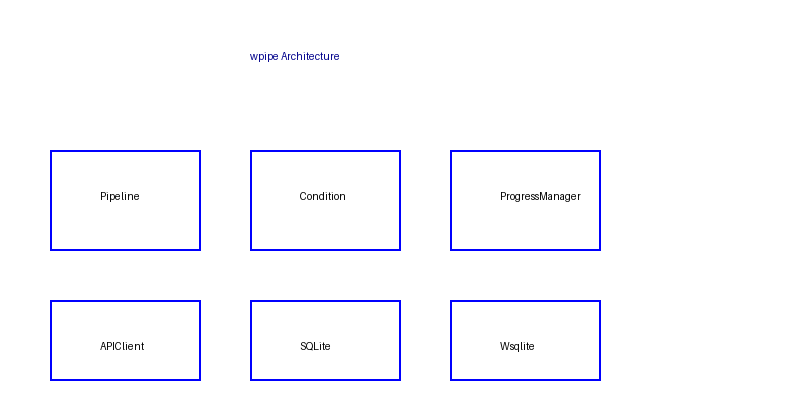
\includegraphics[width=0.9\textwidth]{sources/architecture.png}
    \caption{wpipe System Architecture Overview}
    \label{fig:architecture}
\end{figure}

\section{Core Components}

\subsection{Pipeline Layer}

The Pipeline layer forms the heart of the system, managing step execution and data flow:

\begin{itemize}
    \item \textbf{Pipeline}: Main orchestrator class that manages execution lifecycle
    \item \textbf{Condition}: Handles conditional branching based on data evaluation
    \item \textbf{ProgressManager}: Tracks and displays execution progress
\end{itemize}

\subsection{Integration Layer}

\begin{itemize}
    \item \textbf{APIClient}: Handles HTTP communication with external services
    \item \textbf{Sqlite}: Core database operations for result persistence
    \item \textbf{Wsqlite}: Simplified context manager for database access
\end{itemize}

\subsection{Utilities Layer}

\begin{itemize}
    \item \textbf{new\_logger}: Configured loguru instances for logging
    \item \textbf{memory}: Memory control utilities for resource management
    \item \textbf{leer\_yaml/escribir\_yaml}: YAML configuration management
\end{itemize}

\section{Data Flow Model}

The pipeline operates on an accumulating data model where each step receives all results from previous steps:

\begin{figure}[H]
    \centering
    \begin{tabular}{c}
        \textbf{Input: \{\}} \\
        $\downarrow$ \\
        \textbf{Step 1: \{a: 10\}} \\
        $\downarrow$ \\
        \textbf{Step 2: \{a: 10, b: 20\}} \\
        $\downarrow$ \\
        \textbf{Output: \{a: 10, b: 20, c: 30\}}
    \end{tabular}
    \caption{Data Accumulation Flow}
    \label{fig:dataflow}
\end{figure}

\section{Module Dependencies}

\begin{table}[H]
    \centering
    \\caption{Module Dependency Matrix}
    \label{tab:deps}
    \begin{tabular}{lcccc}
        \toprule
        \textbf{Module} & \textbf{Pipeline} & \textbf{APIClient} & \textbf{SQLite} & \textbf{Logger} \\
        \midrule
        pipe & - & Optional & Optional & Yes \\
        api\_client & Yes & - & No & Yes \\
        sqlite & Yes & No & - & No \\
        exception & Yes & Yes & Yes & No \\
        ram & No & No & No & No \\
        util & No & No & No & No \\
        \bottomrule
    \end{tabular}
\end{table}

% ============================================================================
% CAPÍTULO 3: INSTALACIÓN
% ============================================================================
\chapter{Installation Guide}
\cleardoublepage

\section{Requirements}

Before installing wpipe, ensure your system meets these prerequisites:

\begin{table}[H]
    \centering
    \caption{System Requirements}
    \label{tab:requirements}
    \begin{tabular}{ll}
        \toprule
        \textbf{Component} & \textbf{Requirement} \\
        \midrule
        Python Version & 3.9 or higher \\
        Operating System & Linux, macOS, Windows \\
        Memory & 512 MB minimum \\
        Disk Space & 50 MB \\
        \bottomrule
    \end{tabular}
\end{table}

\section{PyPI Installation (Recommended)}

The simplest installation method uses pip:

\begin{lstlisting}[caption={PyPI Installation}, label={lst:pypi-install}]
pip install wpipe
\end{lstlisting}

Verify the installation:

\begin{lstlisting}[caption={Verification}, label={lst:verify}]
import wpipe
print(wpipe.__version__)
# Output: 1.0.0
\end{lstlisting}

\section{Source Installation}

For development or latest features:

\begin{lstlisting}[caption={Source Installation}, label={lst:source-install}]
git clone https://github.com/wisrovi/wpipe
cd wpipe
pip install -e .
\end{lstlisting}

\section{Development Installation}

Install with all development dependencies for testing and linting:

\begin{lstlisting}[caption={Development Installation}, label={lst:dev-install}]
pip install -e ".[dev]"
\end{lstlisting}

\section{Dependencies}

wpipe has minimal dependencies:

\begin{table}[H]
    \centering
    \caption{Package Dependencies}
    \label{tab:deps-pkg}
    \begin{tabular}{lll}
        \toprule
        \textbf{Package} & \textbf{Version} & \textbf{Purpose} \\
        \midrule
        requests & Any & HTTP client for API integration \\
        pyyaml & Any & YAML configuration parsing \\
        loguru & Any & Logging utilities \\
        rich & Any & Terminal output formatting \\
        \bottomrule
    \end{tabular}
\end{table}

% ============================================================================
% CAPÍTULO 4: GUÍA DE USO
% ============================================================================
\chapter{Usage Guide}
\cleardoublepage

\section{Basic Pipeline}

Creating a simple pipeline requires defining step functions and configuring the Pipeline instance:

\begin{lstlisting}[caption={Basic Pipeline Creation}, label={lst:basic-pipeline}]
from wpipe import Pipeline

def fetch_data(data):
    """Fetch data from source."""
    return {"users": [{"name": "Alice"}, {"name": "Bob"}]}

def process_data(data):
    """Process fetched data."""
    return {"count": len(data["users"])}

def save_data(data):
    """Save results."""
    return {"status": "saved"}

pipeline = Pipeline(verbose=True)
pipeline.set_steps([
    (fetch_data, "Fetch Data", "v1.0"),
    (process_data, "Process Data", "v1.0"),
    (save_data, "Save Data", "v1.0"),
])

result = pipeline.run({})
print(result)
# {'users': [...], 'count': 2, 'status': 'saved'}
\end{lstlisting}

\section{Step Functions}

Step functions receive accumulated data and must return dictionaries:

\begin{lstlisting}[caption={Step Function Definition}, label={lst:step-function}]
def my_step(data):
    # Access data from previous steps
    previous_value = data.get("key", "default")
    
    # Process and return new data
    return {"new_key": previous_value * 2}
\end{lstlisting}

\section{Class-Based Steps}

Classes with \code{\_\_call\_\_} can serve as steps:

\begin{lstlisting}[caption={Class-Based Step}, label={lst:class-step}]
class DataProcessor:
    def __init__(self, multiplier: float):
        self.multiplier = multiplier
        self.count = 0
    
    def __call__(self, data: dict) -> dict:
        self.count += 1
        value = data.get("value", 0)
        return {
            "processed_value": value * self.multiplier,
            "processing_count": self.count,
        }

processor = DataProcessor(multiplier=2.5)
pipeline.set_steps([(processor, "Process", "v1.0")])
\end{lstlisting}

\section{Conditional Pipelines}

The Condition class enables dynamic branching:

\begin{lstlisting}[caption={Conditional Pipeline}, label={lst:condition}]
from wpipe import Pipeline, Condition

def check_value(data):
    return {"value": 75}

def process_high(data):
    return {"result": "High value"}

def process_low(data):
    return {"result": "Low value"}

condition = Condition(
    expression="value > 50",
    branch_true=[(process_high, "High", "v1.0")],
    branch_false=[(process_low, "Low", "v1.0")],
)

pipeline = Pipeline(verbose=True)
pipeline.set_steps([
    (check_value, "Check", "v1.0"),
    condition,
])
\end{lstlisting}

% ============================================================================
% CAPÍTULO 5: INTEGRACIÓN API
% ============================================================================
\chapter{API Integration}
\cleardoublepage

\section{Configuration}

Connect pipelines to external APIs for tracking and monitoring:

\begin{lstlisting}[caption={API Configuration}, label={lst:api-config}]
from wpipe import Pipeline

api_config = {
    "base_url": "https://api.example.com",
    "token": "your-auth-token",
    "timeout": 30,
}

pipeline = Pipeline(api_config=api_config)
pipeline.worker_register(name="processor", version="1.0.0")
\end{lstlisting}

\section{Worker Registration}

Register pipelines as workers for execution tracking:

\begin{lstlisting}[caption={Worker Registration}, label={lst:worker-reg}]
worker_info = pipeline.worker_register(
    name="data_processor",
    version="1.0.0"
)

if worker_info:
    worker_id = worker_info.get("id")
    pipeline.set_worker_id(worker_id)
\end{lstlisting}

\section{Error Handling}

Handle API-related errors gracefully:

\begin{lstlisting}[caption={API Error Handling}, label={lst:api-error}]
from wpipe.exception import ApiError, Codes

try:
    result = pipeline.run(data)
except ApiError as e:
    print(f"API Error: {e}")
    print(f"Code: {e.error_code}")
\end{lstlisting}

% ============================================================================
% CAPÍTULO 6: SQLITE
% ============================================================================
\chapter{SQLite Integration}
\cleardoublepage

\section{Wsqlite Context Manager}

The Wsqlite class provides simplified database access:

\begin{lstlisting}[caption={Wsqlite Usage}, label={lst:wsqlite}]
from wpipe import Pipeline
from wpipe.sqlite import Wsqlite

with Wsqlite(db_name="results.db") as db:
    db.input = {"x": 10}
    result = pipeline.run({"x": 10})
    db.output = result
    print(f"Record ID: {db.id}")
\end{lstlisting}

\section{SQLite Operations}

Core database operations with the Sqlite class:

\begin{lstlisting}[caption={SQLite Operations}, label={lst:sqlite-ops}]
from wpipe.sqlite import Sqlite

db = Sqlite(db_name="results.db")

# Write a record
record_id = db.write(
    input_data={"key": "value"},
    output={"result": "success"},
    details={"version": "1.0"},
    record_id=None
)

# Read by ID
record = db.read_by_id(record_id)

# Export to DataFrame
df = db.export_to_dataframe(save_csv=True, csv_name="records.csv")
\end{lstlisting}

% ============================================================================
% CAPÍTULO 7: MANEJO DE ERRORES
% ============================================================================
\chapter{Error Handling}
\cleardoublepage

\section{Custom Exceptions}

wpipe provides specialized exception types:

\begin{table}[H]
    \centering
    \caption{Exception Classes}
    \label{tab:exceptions}
    \begin{tabular}{lll}
        \toprule
        \textbf{Exception} & \textbf{Code} & \textbf{Usage} \\
        \midrule
        TaskError & 502 & Task execution failure \\
        ApiError & 501 & API communication error \\
        ProcessError & 504 & Process update failure \\
        Codes & - & Error code constants \\
        \bottomrule
    \end{tabular}
\end{table}

\section{Error Codes}

\begin{lstlisting}[caption={Error Codes}, label={lst:error-codes}]
from wpipe.exception import TaskError, Codes

try:
    result = pipeline.run(data)
except TaskError as e:
    print(f"Error Code: {e.error_code}")
    print(f"Message: {str(e)}")
\end{lstlisting}

\section{Best Practices}

\begin{itemize}
    \item Validate input early in the pipeline
    \item Use descriptive error messages
    \item Implement retry logic for transient failures
    \item Log errors with context for debugging
    \item Provide fallback behaviors when possible
\end{itemize}

% ============================================================================
% CAPÍTULO 8: CONFIGURACIÓN
% ============================================================================
\chapter{Configuration}
\cleardoublepage

\section{YAML Configuration}

Load pipeline configuration from YAML files:

\begin{lstlisting}[caption={YAML Loading}, label={lst:yaml-load}]
from wpipe.util import leer_yaml

config = leer_yaml("config.yaml")
pipeline = Pipeline(**config["pipeline"])
pipeline.set_steps(config["steps"])
\end{lstlisting}

\section{Environment Variables}

Access environment variables in configuration:

\begin{lstlisting}[caption={Environment Variables}, label={lst:env}]
import os

api_config = {
    "base_url": os.environ["API_URL"],
    "token": os.environ["API_TOKEN"],
}
\end{lstlisting}

% ============================================================================
% CAPÍTULO 9: CASOS DE USO
% ============================================================================
\chapter{Use Cases}
\cleardoublepage

\section{ETL Pipelines}

Extract, Transform, Load workflows:

\begin{lstlisting}[caption={ETL Pipeline}, label={lst:etl}]
def extract(data):
    return {"raw_data": fetch_from_api()}

def transform(data):
    cleaned = clean_data(data["raw_data"])
    return {"transformed": enriched_data}

def load(data):
    save_to_database(data["transformed"])
    return {"status": "loaded"}
\end{lstlisting}

\section{Data Validation}

Input validation with error handling:

\begin{lstlisting}[caption={Validation Pipeline}, label={lst:validation}]
def validate_input(data):
    required_fields = ["email", "name", "age"]
    for field in required_fields:
        if field not in data:
            raise TaskError(
                f"Missing: {field}",
                step_name="Validate Input",
                code=Codes.TASK_FAILED
            )
    return {"validated": True}
\end{lstlisting}

\section{Machine Learning Pipelines}

ML model inference workflows:

\begin{lstlisting}[caption={ML Pipeline}, label={lst:ml-pipeline}]
def load_model(data):
    model = load_pytorch_model("model.pth")
    return {"model": model, "input": data["input"]}

def preprocess(data):
    tensor = transform(data["input"])
    return {"tensor": tensor}

def predict(data):
    output = data["model"](data["tensor"])
    return {"prediction": output.tolist()}
\end{lstlisting}

% ============================================================================
% CAPÍTULO 10: MÉTRICAS
% ============================================================================
\chapter{Performance Metrics}
\cleardoublepage

\section{Quality Metrics}

wpipe maintains high code quality standards:

\begin{table}[H]
    \centering
    \caption{Code Quality Metrics}
    \label{tab:metrics}
    \begin{tabular}{lr}
        \toprule
        \textbf{Metric} & \textbf{Value} \\
        \midrule
        Total Tests & 106 passing \\
        Examples & 100+ \\
        Type Hints & 100\% \\
        Python Support & 3.9, 3.10, 3.11, 3.12, 3.13 \\
        Documentation Pages & 35+ \\
        \bottomrule
    \end{tabular}
\end{table}

\section{Test Coverage}

Run tests with coverage reporting:

\begin{lstlisting}[caption={Test Coverage}, label={lst:coverage}]
pytest --cov=wpipe --cov-report=html
open htmlcov/index.html
\end{lstlisting}

\section{Quality Checks}

Comprehensive quality validation:

\begin{lstlisting}[caption={Quality Checks}, label={lst:quality}]
# Linting
ruff check wpipe/

# Type checking
mypy wpipe/

# All checks
ruff check wpipe/ && mypy wpipe/ && pytest
\end{lstlisting}

% ============================================================================
% CAPÍTULO 11: MEJORES PRÁCTICAS
% ============================================================================
\chapter{Best Practices}
\cleardoublepage

\section{Design Principles}

\begin{enumerate}
    \item \textbf{Keep steps focused}: Each step should perform one logical operation
    \item \textbf{Return dictionaries}: Steps must always return dict objects
    \item \textbf{Handle missing keys}: Use \code{.get()} with defaults
    \item \textbf{Use descriptive names}: Clear step names aid debugging
    \item \textbf{Version your steps}: Track changes with version strings
\end{enumerate}

\section{Code Organization}

\begin{lstlisting}[caption={Code Organization}, label={lst:organization}]
# Good: Focused, descriptive steps
pipeline.set_steps([
    (fetch_users, "Fetch Users from Database", "v1.0"),
    (validate_emails, "Validate Email Addresses", "v1.0"),
    (send_notifications, "Send Welcome Emails", "v1.0"),
])

# Bad: Vague names
pipeline.set_steps([
    (step1, "Step 1", "v1.0"),
    (step2, "Step 2", "v1.0"),
])
\end{lstlisting}

\section{Error Handling Patterns}

\begin{lstlisting}[caption={Error Handling Pattern}, label={lst:error-pattern}]
def robust_step(data):
    try:
        result = unreliable_operation()
        return {"result": result}
    except SpecificError:
        return {"result": "fallback"}
    except Exception as e:
        raise TaskError(
            f"Operation failed: {e}",
            step_name="Robust Step",
            code=Codes.TASK_FAILED
        )
\end{lstlisting}

% ============================================================================
% CAPÍTULO 12: TROUBLESHOOTING
% ============================================================================
\chapter{Troubleshooting}
\cleardoublepage

\section{Common Issues}

\subsection{ImportError}

\begin{itemize}
    \item Ensure wpipe is installed: \code{pip install wpipe}
    \item Verify Python path includes site-packages
    \item Check for virtual environment activation
\end{itemize}

\subsection{KeyError in Steps}

\begin{itemize}
    \item Use \code{.get()} with defaults for optional data
    \item Validate required keys exist before accessing
    \item Check step execution order
\end{itemize}

\subsection{TypeError in Steps}

\begin{itemize}
    \item Ensure steps return dictionaries
    \item Verify data types match expectations
    \item Add type hints for better error messages
\end{itemize}

\section{Debugging Techniques}

\begin{lstlisting}[caption={Verbose Output}, label={lst:debug}]
pipeline = Pipeline(verbose=True)
result = pipeline.run(data, verbose=True)
\end{lstlisting}

\section{Logging Configuration}

\begin{lstlisting}[caption={Logging Setup}, label={lst:logging}]
from wpipe.log import new_logger

logger = new_logger(
    process_name="my_pipeline",
    path_file="./logs",
    filename_format="{time:YYYY-MM-DD}"
)
logger.info("Pipeline started")
\end{lstlisting}

% ============================================================================
% CAPÍTULO 13: CONCLUSIONES
% ============================================================================
\chapter{Conclusions and Future Work}
\cleardoublepage

\section{Summary}

wpipe provides a powerful yet lightweight solution for sequential data processing pipelines. Key achievements include:

\begin{itemize}
    \item Simplified pipeline orchestration without complex infrastructure
    \item Comprehensive error handling and retry mechanisms
    \item Extensive documentation with 100+ examples
    \item Production-ready with 106 passing tests
    \item Minimal dependencies for easy deployment
\end{itemize}

\section{Future Enhancements}

Potential areas for future development:

\begin{enumerate}
    \item Parallel execution support for independent steps
    \item Distributed execution across multiple workers
    \item Additional database backend support
    \item Web-based monitoring dashboard
    \item Graphical pipeline builder
\end{enumerate}

\section{Contributing}

Contributions are welcome. Please visit the GitHub repository for guidelines.

% ============================================================================
% BIBLIOGRAFÍA
% ============================================================================
\chapter{Bibliography}
\cleardoublepage

\begin{thebibliography}{99}
\sffamily

bibitem{python} Python Software Foundation. \textit{Python Programming Language}. https://www.python.org/

bibitem{requests} Kenneth Reitz. \textit{Requests: HTTP for Humans}. https://docs.python-requests.org/

bibitem{loguru} Loguru Authors. \textit{Loguru}. https://loguru.readthedocs.io/

bibitem{rich} Textualize. \textit{Rich}. https://rich.readthedocs.io/

bibitem{pyyaml} PyYAML Developers. \textit{PyYAML}. https://pyyaml.org/

bibitem{pytest} pytest developers. \textit{pytest}. https://docs.pytest.org/

bibitem{ruff} Astral. \textit{Ruff}. https://docs.astral.sh/ruff/

bibitem{mypy} mypy developers. \textit{mypy}. https://mypy.readthedocs.io/

bibitem{sphinx} Sphinx developers. \textit{Sphinx Documentation Generator}. https://www.sphinx-doc.org/

bibitem{airflow} Apache Airflow. \textit{Airflow Platform}. https://airflow.apache.org/

bibitem{prefect} Prefect. \textit{Prefect Workflow Engine}. https://www.prefect.io/

bibitem{dagster} Dagster. \textit{Dagster Data Asset Pipeline}. https://dagster.io/

\end{thebibliography}

% ============================================================================
% APÉNDICES
% ============================================================================
\begin{appendices}
\chapter{Advanced Configurations}
\cleardoublepage

\section{Retry Configuration}

Configure automatic retries with exponential backoff:

\begin{lstlisting}[caption={Retry Configuration}, label={lst:retry-config}]
pipeline = Pipeline(
    verbose=True,
    max_retries=3,
    retry_delay=2.0,
    retry_on_exceptions=(ConnectionError, TimeoutError),
)
\end{lstlisting}

\section{Memory Control}

Limit memory usage on Linux systems:

\begin{lstlisting}[caption={Memory Control}, label={lst:memory}]
from wpipe.ram import memory, memory_limit

# Set memory limit
memory_limit(percentage=0.8)

# Decorator usage
@memory(percentage=0.5)
def memory_intensive_function():
    pass
\end{lstlisting}

\section{Nested Pipelines}

Compose complex workflows from smaller pipelines:

\begin{lstlisting}[caption={Nested Pipeline}, label={lst:nested}]
sub_pipeline = Pipeline()
sub_pipeline.set_steps([
    (step_a, "Step A", "v1.0"),
    (step_b, "Step B", "v1.0"),
])

main_pipeline = Pipeline()
main_pipeline.set_steps([
    (sub_pipeline.run, "Run Sub-pipeline", "v1.0"),
    (step_c, "Step C", "v1.0"),
])
\end{lstlisting}

\chapter{API Reference}
\cleardoublepage

\section{Pipeline Class}

\begin{lstlisting}[caption={Pipeline Initialization}, label={lst:pipeline-init}]
class Pipeline:
    def __init__(
        self,
        worker_id: Optional[str] = None,
        worker_name: str = "worker",
        api_config: Optional[dict] = None,
        verbose: bool = False,
        max_retries: int = 0,
        retry_delay: float = 1.0,
        retry_on_exceptions: tuple = (Exception,),
    ): ...
\end{lstlisting}

\section{Condition Class}

\begin{lstlisting}[caption={Condition Initialization}, label={lst:condition-init}]
class Condition:
    def __init__(
        self,
        expression: str,
        branch_true: list,
        branch_false: Optional[list] = None,
    ): ...
\end{lstlisting}

\chapter{Example Scripts}
\cleardoublepage

\section{Basic Example}

Complete working example with all features:

\begin{lstlisting}[caption={Complete Example}, label={lst:complete}]
"""
Complete wpipe Example
"""
from wpipe import Pipeline, Condition

def fetch_data(data):
    return {"numbers": [1, 2, 3, 4, 5]}

def calculate_sum(data):
    return {"sum": sum(data["numbers"])}

def calculate_average(data):
    return {"average": data["sum"] / len(data["numbers"])}

def format_result(data):
    return {"output": f"Sum={data['sum']}, Avg={data['average']}"}

if __name__ == "__main__":
    pipeline = Pipeline(verbose=True)
    pipeline.set_steps([
        (fetch_data, "Fetch Data", "v1.0"),
        (calculate_sum, "Calculate Sum", "v1.0"),
        (calculate_average, "Calculate Average", "v1.0"),
        (format_result, "Format Result", "v1.0"),
    ])
    
    result = pipeline.run({})
    print(result)
\end{lstlisting}

\end{appendices}

% ============================================================================
% PÁGINA DE AGRADECIMIENTO
% ============================================================================
\cleardoublepage
\thispagestyle{empty}
\vspace*{3cm}

\begin{center}
{\color{blue!70!black}\Huge\textbf{\sffamily Thank You}}\\[2cm]

{\large\sffamily
Thank you for choosing wpipe for your data processing needs.}\\[0.5cm]

{\large\sffamily
Your feedback and contributions help improve this library for everyone.}\\[1.5cm]

{\Large\sffamily\textbf{Get Started:}}\\[0.5cm]

\fbox{
    \parbox{0.8\textwidth}{
        \centering\sffamily
        \href{https://github.com/wisrovi/wpipe}{GitHub: github.com/wisrovi/wpipe}\\[0.3cm]
        \href{https://wpipe.readthedocs.io}{Documentation: wpipe.readthedocs.io}\\[0.3cm]
        \href{https://pypi.org/project/wpipe}{PyPI: pypi.org/project/wpipe}
    }
}
\\[2cm]

{\large\sffamily
Questions? Issues? Contributions?}\\[0.5cm]

{\large\sffamily
We welcome all feedback and contributions!}
\end{center}

\vfill

\begin{center}
{\small\sffamily
Copyright \copyright\ 2024 William Steve Rodriguez Villamizar}\\
{\small\sffamily
MIT License}
\end{center}

\end{document}
